\chapter{QR Factorization}

\begin{definition}[Lower Triangular Matrices]
    矩阵 $ \mathrm{A} \in \mathbb{R}^{n \times n} $ 为\term{下三角(Lower Triangular)矩阵}, $ A_{i j}=0, j>i $ 。

    $$ A=\left[\begin{array}{ccccc}A_{11} & 0 & \cdots & 0 & 0 \\ A_{21} & A_{22} & \cdots & 0 & 0 \\ \vdots & \vdots & \ddots & \vdots & \vdots \\ A_{n-1,1} & A_{n-1,2} & \cdots & A_{n-1, n-1} & 0 \\ A_{n 1} & A_{n 2} & \cdots & A_{n, n-1} & A_{n n}\end{array}\right] $$
\end{definition}

\begin{definition}[Upper Triangular Matrices]
    $ A^{T} $ 为\term{上三角(Upper Triangular)矩阵}。

    $$ A=\left[\begin{array}{ccccc}A_{11} & A_{12} & \cdots & A_{1, n-1} & A_{1, n} \\ 0 & A_{22} & \cdots & A_{2, n-1} & A_{2, n} \\ \vdots & \vdots & \ddots & \vdots & \vdots \\ 0 & 0 & \cdots & A_{n-1, n-1} & A_{n-1, n} \\ 0 & 0 & \cdots & 0 & A_{n n}\end{array}\right] $$
\end{definition}

\begin{definition}[单位上三角矩阵,单位下三角矩阵]
    对角元素 $ a_{i i} $ 都等于 1的上(下)三角矩阵。
\end{definition}

\section{高斯消元法}

\begin{problem}
    当 $ A $ 是具有非零对角元素的下三角矩阵时,解 $ A x=b $ 。
\end{problem}

使用前向回代(Forward Substitution)算法求解。

时间复杂度: $ 1+3+5+\ldots+(2 \mathrm{n}-1)=\mathrm{n}^{2} $ flops

\begin{algorithm}[htbp]
    \caption{Forward Substitution}
    $ x_{1}= \frac{b_{1} }{A_{11} }  $\;
$ x_{2}=\frac{b_{2}-A_{21} x_{1}}{A_{22}}$\;
$  x_{3} =\frac{b_{3}-A_{31} x_{1}-A_{32} x_{2}}{A_{33}} $ \;
    $\cdots$  \;
    $x_{n} =
    \frac{b_{n}-A_{n 1} x_{1}-A_{n 2} x_{2}-\cdots-A_{n, n-1} x_{n-1}}{A_{n n}} $\;
\end{algorithm}

\begin{problem}
    当A是具有非零对角元素的上三角矩阵, 解 $ \mathrm{A} x=\mathrm{b} $ 。
\end{problem}

使用后向回代(Back Substitution)算法来求解.

\begin{algorithm}[htbp]
    \caption{Backward Substitution}

    $ x_{n}= \frac{b_{n}}{A_{n n}} $\;
    $ x_{n-1}= \frac{b_{n-1}-A_{n-1, n} x_{n}}{A_{n-1, n-1}} $ \;
    $ x_{n-2}= \frac{b_{n-2}-A_{n-2, n-1} x_{n-1}-A_{n-2, n} x_{n}}{ A_{n-2, n-2}} $\;
    $\cdots$\;
    $ x_{1}=\frac{b_{1}-A_{12} x_{2}-A_{13} x_{3}-\cdots-A_{1 n} x_{n}}{A_{11}}  $\;
\end{algorithm}

时间复杂度: $ 1+3+\ldots+2 \mathrm{n}-1=\mathrm{n}^{2} $ flops

\begin{theorem}
    对角元素非零的三角矩阵A是非奇异的,即:
$$
A x=0 \quad \Rightarrow \quad x=0
$$
\end{theorem}

\begin{theorem}[高斯消元法]
    $A$的逆可以通过逐列解方程$AX=I$来计算得到

    $$ A\left[\begin{array}{llll}x_{1} & x_{2} & \cdots & x_{n}\end{array}\right]=\left[\begin{array}{llll}e_{1} & e_{2} & \cdots & e_{n}\end{array}\right] $$
\end{theorem}

\begin{theorem}
    下三角矩阵的逆是下三角矩阵,上三角矩阵的逆是上三角矩阵。
\end{theorem}

上/下三角矩阵 $ \mathrm{A} \in \mathbb{R}^{n \times n} $ 逆的复杂度

$$ n^{2}+(n-1)^{2}+\cdots+1 \approx \frac{1}{3} n^{3}\text{ flops }$$ 

\section{QR Factorization}

如果矩阵 $ A \in \mathbb{R}^{m \times n} $ 的列向量线性无关,则可以将其分解为

\begin{definition}[QR Factorization]
    
    $$\begin{aligned} A&=\left[\begin{array}{llll}a_{1} & a_{2} & \cdots & a_{n}\end{array}\right]\\
    &=\left[\begin{array}{llll}q_{1} & q_{2} & \cdots & q_{n}\end{array}\right]\left[\begin{array}{cccc}R_{11} & R_{12} & \cdots & R_{1 n} \\ 0 & R_{22} & \cdots & R_{2 n} \\ \vdots & \vdots & \ddots & \vdots \\ 0 & 0 & \cdots & R_{n n}\end{array}\right]\\
    &=QR
    \end{aligned}$$

向量 $ q_{1}, \ldots, q_{n} \in \mathbb{R}^{m} $ 是标准正交向量:
$$
\left\|q_{i}\right\|_{2}=1, \quad q_{i}^{T} q_{j}=0, \text { if } \quad i \neq j
$$

对角元素 $ R_{i i} $ 是非零的。若 $ R_{i i}<0 $, 改变 $ R_{i i}, \cdots, R_{i n} $ 和向量 $ q_{i} $ 的符号。大多数定义要求 $ R_{i i}>0 $,使得$Q$和$R$是唯一的。
\end{definition}

QR分解依赖于Gram-Schmidit正交化法。(参见\ref{Chap:Gram-Schmidt Algorithm}).QR分解的思想可以用于加快求逆矩阵速度。

$$\begin{aligned}
   Ax = b &\Rightarrow x = A^{-1} b \\
QRx = b &\Rightarrow x = R^{-1} \left(Q^Tb\right)
\end{aligned}
$$

\begin{remark}
    Gram-Schmidt(正交化) $$ \quad \widetilde{q}_{i}=a_{i}-\left(q_{1}^{T} a_{i}\right) q_{1}-\cdots-\left(q_{i-1}^{T} a_{i}\right) q_{i-1} $$

    $$ \begin{aligned}
        a_{i}&=\left(q_{1}^{T} a_{i}\right) q_{1}+\cdots+\left(q_{i-1}^{T} a_{i}\right) q_{i-1} + \left\|\tilde{q}_{i}\right\|_{2} q_{i}
        \\ &=R_{1 i} q_{1}+\cdots+R_{i i} q_{i}
    \end{aligned}
      $$
\end{remark}

\begin{corollary}
    $ Q \in \mathbb{R}^{m \times n} $ 具有标准正交列 $ \left(Q^{T} Q=I\right) $.
\end{corollary}

\begin{corollary}
    如果 $ A $ 是方阵 $ (\mathrm{m}=\mathrm{n}) $, 则 $ Q $ 是正交的 $ \left(Q^{T} Q=Q Q^{T}=I\right) $.
\end{corollary}

\begin{corollary}
    $ R \in \mathbb{R}^{n \times n} $ 的上三角矩阵.
\end{corollary}

\begin{corollary}
     $ R $ 是非奇异的(对角元素是非零的).
\end{corollary}

\begin{algorithm}[htbp]
    \caption{QR Decompostion Algorithm}
    
    设矩阵 $ A $ 的列向量依次为 $ a_{1}, a_{2}, \cdots, a_{n} $ ,由于 $ A $ 为非奇异矩阵, 则列向量线性无关\;
    对列向量 $ a_{1}, a_{2}, \ldots, a_{n} $ 按照Gram-Schmidt方法进行正交化,然后单位化\;
    单位化得到的标准正交向量 $ q_{1}, q_{2}, \ldots, q_{n} $, 即得到标准正交矩阵$Q$\;
    根据 $ R=Q^{-1} A \Rightarrow R=Q^{T} A $, 得到上三角矩阵$R$\;
    $ Q R $ 分解 $ A=Q R $\;
\end{algorithm}

\begin{example}
    矩阵$A$的QR分解过程

    $$ A=\left[\begin{array}{ccc}1 & 1 & 0 \\ 1 & -1 & 1 \\ 0 & 0 & 2\end{array}\right] $$

    令 $ a_{1}=(1,1,0)^{T}, a_{2}=(1,-1,0)^{T}, a_{3}=(0,1,2)^{T} $, 由Schmidt方法正交单 位化后, 得到 $ q_{1}=\left(\frac{1}{\sqrt{2}}, \frac{1}{\sqrt{2}}, 0\right)^{T}, q_{2}=\left(\frac{1}{\sqrt{2}},-\frac{1}{\sqrt{2}}, 0\right)^{T}, q_{3}=(0,0,1)^{T} $ 。

    所以 $ a_{1}=\sqrt{2} q_{1}, \quad a_{2}=\sqrt{2} q_{2}, \quad a_{3}=\frac{1}{\sqrt{2}} q_{1}-\frac{1}{\sqrt{2}} q_{2}+2 q_{3} $ 。

    $$ A=Q R=\left[\begin{array}{ccc}\frac{1}{\sqrt{2}} & \frac{1}{\sqrt{2}} & 0 \\ \frac{1}{\sqrt{2}} & -\frac{1}{\sqrt{2}} & 0 \\ 0 & 0 & 1\end{array}\right]\left[\begin{array}{ccc}\sqrt{2} & 0 & \frac{1}{\sqrt{2}} \\ 0 & \sqrt{2} & -\frac{1}{\sqrt{2}} \\ 0 & 0 & 2\end{array}\right] $$

    $$ \begin{aligned}\left[\begin{array}{rrr}-1 & -1 & 1 \\ 1 & 3 & 3 \\ -1 & -1 & 5 \\ 1 & 3 & 7\end{array}\right] &=\left[\begin{array}{rrr}-1 / 2 & 1 / 2 & -1 / 2 \\ 1 / 2 & 1 / 2 & -1 / 2 \\ -1 / 2 & 1 / 2 & 1 / 2 \\ 1 / 2 & 1 / 2 & 1 / 2\end{array}\right]\left[\begin{array}{ccc}2 & 4 & 2 \\ 0 & 2 & 8 \\ 0 & 0 & 4\end{array}\right] \\ &=\left[\begin{array}{lll}q_{1} & q_{2} & q_{3}\end{array}\right]\left[\begin{array}{ccc}R_{11} & R_{12} & R_{13} \\ 0 & R_{22} & R_{23} \\ 0 & 0 & R_{33}\end{array}\right] \\ &=Q R \end{aligned} $$
\end{example}

\begin{example}
    $$
\begin{aligned}
\left[\begin{array}{rrr}
-1 & -1 & 1 \\
1 & 3 & 3 \\
-1 & -1 & 5 \\
1 & 3 & 7
\end{array}\right] &=\left[\begin{array}{rrr}
-1 / 2 & 1 / 2 & -1 / 2 \\
1 / 2 & 1 / 2 & -1 / 2 \\
-1 / 2 & 1 / 2 & 1 / 2 \\
1 / 2 & 1 / 2 & 1 / 2
\end{array}\right]\left[\begin{array}{rrr}
2 & 4 & 2 \\
0 & 2 & 8 \\
0 & 0 & 4
\end{array}\right] \\
&=\left[\begin{array}{lll}
q_{1} & q_{2} & q_{3}
\end{array}\right]\left[\begin{array}{ccc}
R_{11} & R_{12} & R_{13} \\
0 & R_{22} & R_{23} \\
0 & 0 & R_{33}
\end{array}\right] \\
&=Q R
\end{aligned}
$$
\end{example}

\section{QR分解的应用}

可用QR分解求解以下问题:

\begin{itemize}
    \item 线性方程
    \item 最小二乘问题
    \item 带约束的最小二乘问题
\end{itemize}

\subsection{QR分解和伪逆、逆}

\begin{definition}[线性无关列向量的矩阵$A$的伪逆]
    $$A^{\dagger}=\left(A^{T} A\right)^{-1} A^{T}$$
\end{definition}

\begin{theorem}
    $$
\begin{aligned}
A^{\dagger}&=\left((Q R)^{T}(Q R)\right)^{-1}(Q R)^{T} \\
&=\left(R^{T} Q^{T} Q R\right)^{-1} R^{T} Q^{T} \\
&=\left(R^{T} R\right)^{-1} R^{T} Q^{T} \quad\left(Q^{T} Q=I\right) \\
&=R^{-1} R^{-T} R^{T} Q^{T} \quad(R{\text {是非奇异的 })} \\
 &={R^{-1} Q^{T}}
\end{aligned}
$$
\end{theorem}

\begin{corollary}
    对于方阵非奇异矩阵 $\mathrm{A}$, 其逆为
$$
A^{-1}=(Q R)^{-1}=R^{-1} Q^{T}
$$
\end{corollary}

\subsection{$A$的列空间与$Q$的关系}

矩阵 $A \in \mathbb{R}^{m \times n}$ 的值域范围定义为:
$$
\operatorname{range}(A)=\left\{A x \mid x \in \mathbf{R}^{n}\right\}
$$

\begin{theorem}
    假设$A$有线性无关的列向量,且其QR因子为 $Q, R$

    $Q$ 和 $A$ 的值域范围相同(有相同的列空间)。

\end{theorem}

即$Q$ 的列向量是标准正交的,并且和 $A$ 的列向量张成相同的空间。

\begin{proof}
    $$
\begin{aligned}
y \in \operatorname{range}(A) & \Leftrightarrow \quad y=A x, x \in \mathbb{R}^{n} \\
\Leftrightarrow & y=Q R x, z=R x \\
& \Leftrightarrow \quad y=Q z, z \in \mathbb{R}^{n} \\
& \Leftrightarrow \quad y \in \operatorname{range}(Q)
\end{aligned}
$$
\end{proof}

\subsection{往$A$列空间上的投影}

结合 $A=Q R$ 和 $A^{\dagger}=R^{-1} Q^{T}$, 可得:

$$
A A^{\dagger}=Q R R^{-1} Q^{T}=Q Q^{T}
$$

\begin{remark}
    注意在 $A A^{\dagger}$ 中乘积的顺序与 $A^{\dagger} A=$ 的差异。
\end{remark}

$$
\begin{aligned}
&\min _{y}\|Q y-x\|_{2}^{2}\\
 \Rightarrow& Q^{T}(Q y-x)=0 \\
\Rightarrow& Q^{T} Q y=Q^{T} x\\ 
\Rightarrow & y=Q^{T} x
\end{aligned}
$$

$Q Q^{T} x$ 是 $x$ 在 $Q$ 值域上的投影



\tikzset{every picture/.style={line width=0.75pt}} %set default line width to 0.75pt        

\begin{figure}[htbp]
    \begin{tikzpicture}[x=0.75pt,y=0.75pt,yscale=-1,xscale=1]
%uncomment if require: \path (0,300); %set diagram left start at 0, and has height of 300

%Shape: Parallelogram [id:dp16734778977883136] 
\draw  [color={rgb, 255:red, 255; green, 255; blue, 255 }  ,draw opacity=1 ][fill={rgb, 255:red, 179; green, 179; blue, 179 }  ,fill opacity=1 ] (224.15,98.88) -- (563.14,98.88) -- (417.85,242.95) -- (78.86,242.95) -- cycle ;
%Straight Lines [id:da3519715103345966] 
\draw [color={rgb, 255:red, 0; green, 0; blue, 0 }  ,draw opacity=1 ][line width=1.5]  [dash pattern={on 1.69pt off 2.76pt}]  (399.96,59.43) -- (399.07,151.88) ;
%Straight Lines [id:da7143500773565701] 
\draw [color={rgb, 255:red, 74; green, 144; blue, 226 }  ,draw opacity=1 ][line width=2.25]    (252.07,166.88) -- (395.92,62.37) ;
\draw [shift={(399.96,59.43)}, rotate = 504] [fill={rgb, 255:red, 74; green, 144; blue, 226 }  ,fill opacity=1 ][line width=0.08]  [draw opacity=0] (14.29,-6.86) -- (0,0) -- (14.29,6.86) -- cycle    ;
%Straight Lines [id:da29623635442698415] 
\draw [color={rgb, 255:red, 234; green, 81; blue, 100 }  ,draw opacity=1 ][line width=2.25]    (252.07,166.88) -- (394.09,152.39) ;
\draw [shift={(399.07,151.88)}, rotate = 534.1700000000001] [fill={rgb, 255:red, 234; green, 81; blue, 100 }  ,fill opacity=1 ][line width=0.08]  [draw opacity=0] (14.29,-6.86) -- (0,0) -- (14.29,6.86) -- cycle    ;

% Text Node
\draw (114.72,185.99) node [anchor=north west][inner sep=0.75pt]    {$\begin{aligned}
C( A) & =C( Q)\\
\operatorname{range}( A) & =\operatorname{range}( Q)
\end{aligned}$};
% Text Node
\draw (376.21,43.4) node [anchor=north west][inner sep=0.75pt]    {$x$};
% Text Node
\draw  [color={rgb, 255:red, 0; green, 0; blue, 0 }  ,draw opacity=0 ][fill={rgb, 255:red, 234; green, 81; blue, 100 }  ,fill opacity=1 ]  (347.57,167.38) .. controls (347.57,164.62) and (349.8,162.38) .. (352.57,162.38) -- (463.57,162.38) .. controls (466.33,162.38) and (468.57,164.62) .. (468.57,167.38) -- (468.57,182.38) .. controls (468.57,185.14) and (466.33,187.38) .. (463.57,187.38) -- (352.57,187.38) .. controls (349.8,187.38) and (347.57,185.14) .. (347.57,182.38) -- cycle  ;
\draw (350.57,166.78) node [anchor=north west][inner sep=0.75pt]    {$AA^{\dagger } x=QQ^{T} x$};


\end{tikzpicture}
\end{figure}


\tikzset{every picture/.style={line width=0.75pt}} %set default line width to 0.75pt        
\begin{figure}[htbp]

    \caption{$ A \boldsymbol{x}^{+} $ in the column space goes back to $ A^{+} A \boldsymbol{x}^{+}=\boldsymbol{x}^{+} $in the row space}
\begin{tikzpicture}[x=0.75pt,y=0.75pt,yscale=-1,xscale=1]
%uncomment if require: \path (0,378); %set diagram left start at 0, and has height of 378

%Shape: Rectangle [id:dp8596899930926358] 
\draw  [dash pattern={on 0.84pt off 2.51pt}] (412.64,146.65) -- (440.94,174.46) -- (412.24,203.67) -- (383.93,175.86) -- cycle ;
%Shape: Rectangle [id:dp144129295466213] 
\draw   (159.81,65.14) -- (236.34,135.27) -- (193.59,181.93) -- (117.06,111.79) -- cycle ;
%Shape: Rectangle [id:dp4244539260616451] 
\draw   (193.59,181.93) -- (260.03,242.81) -- (218.64,287.99) -- (152.2,227.1) -- cycle ;

%Shape: Rectangle [id:dp10811540545272225] 
\draw   (477.03,51.53) -- (398.27,133.34) -- (440.51,174) -- (519.26,92.19) -- cycle ;
%Shape: Rectangle [id:dp952165170642489] 
\draw   (440.51,174) -- (372.14,245.02) -- (413.05,284.39) -- (481.41,213.38) -- cycle ;

%Straight Lines [id:da43480021093829335] 
\draw [color={rgb, 255:red, 139; green, 87; blue, 42 }  ,draw opacity=1 ][line width=2.25]    (193.59,181.93) -- (187.34,138.27) ;
\draw [shift={(186.64,133.33)}, rotate = 441.85] [fill={rgb, 255:red, 139; green, 87; blue, 42 }  ,fill opacity=1 ][line width=0.08]  [draw opacity=0] (8.57,-4.12) -- (0,0) -- (8.57,4.12) -- cycle    ;
%Straight Lines [id:da6356667569876433] 
\draw [color={rgb, 255:red, 245; green, 166; blue, 35 }  ,draw opacity=1 ][line width=2.25]    (440.51,175) -- (415.75,200.11) ;
\draw [shift={(412.24,203.67)}, rotate = 314.6] [fill={rgb, 255:red, 245; green, 166; blue, 35 }  ,fill opacity=1 ][line width=0.08]  [draw opacity=0] (8.57,-4.12) -- (0,0) -- (8.57,4.12) -- cycle    ;
%Straight Lines [id:da22563123154133025] 
\draw [color={rgb, 255:red, 65; green, 117; blue, 5 }  ,draw opacity=1 ][line width=2.25]    (440.51,175) -- (388.93,175.78) ;
\draw [shift={(383.93,175.86)}, rotate = 359.13] [fill={rgb, 255:red, 65; green, 117; blue, 5 }  ,fill opacity=1 ][line width=0.08]  [draw opacity=0] (8.57,-4.12) -- (0,0) -- (8.57,4.12) -- cycle    ;
%Shape: Rectangle [id:dp12172823301153524] 
\draw   (186.5,176.41) -- (193.59,182.93) -- (186.84,190.28) -- (179.74,183.76) -- cycle ;
%Shape: Rectangle [id:dp9349834759264539] 
\draw   (447.27,167.65) -- (454.36,174.17) -- (447.61,181.52) -- (440.51,175) -- cycle ;
%Straight Lines [id:da2510398254796229] 
\draw [color={rgb, 255:red, 108; green, 108; blue, 215 }  ,draw opacity=1 ][line width=2.25]    (440.51,175) -- (416.14,150.21) ;
\draw [shift={(412.64,146.65)}, rotate = 405.49] [fill={rgb, 255:red, 108; green, 108; blue, 215 }  ,fill opacity=1 ][line width=0.08]  [draw opacity=0] (8.57,-4.12) -- (0,0) -- (8.57,4.12) -- cycle    ;
%Straight Lines [id:da5471202445204062] 
\draw  [dash pattern={on 4.5pt off 4.5pt}]  (383.93,175.86) -- (186.64,133.33) ;
\draw [shift={(285.28,154.59)}, rotate = 372.15999999999997] [fill={rgb, 255:red, 0; green, 0; blue, 0 }  ][line width=0.08]  [draw opacity=0] (8.93,-4.29) -- (0,0) -- (8.93,4.29) -- cycle    ;
%Straight Lines [id:da12114390650727058] 
\draw  [dash pattern={on 4.5pt off 4.5pt}]  (412.64,146.65) -- (186.64,133.33) ;
\draw [shift={(299.64,139.99)}, rotate = 363.37] [fill={rgb, 255:red, 0; green, 0; blue, 0 }  ][line width=0.08]  [draw opacity=0] (8.93,-4.29) -- (0,0) -- (8.93,4.29) -- cycle    ;
%Straight Lines [id:da8219115744539653] 
\draw  [dash pattern={on 4.5pt off 4.5pt}]  (412.24,203.67) -- (193.59,181.93) ;
\draw [shift={(302.92,192.8)}, rotate = 365.68] [fill={rgb, 255:red, 0; green, 0; blue, 0 }  ][line width=0.08]  [draw opacity=0] (8.93,-4.29) -- (0,0) -- (8.93,4.29) -- cycle    ;

% Text Node
\draw (74,15) node [anchor=north west][inner sep=0.75pt]   [align=left] {Row Space $\displaystyle A^{T} y$\\dim $\displaystyle r$};
% Text Node
\draw (63,299) node [anchor=north west][inner sep=0.75pt]   [align=left] {Nullspace $\displaystyle Ax=0$\\dim $\displaystyle n-r$};
% Text Node
\draw (434,8) node [anchor=north west][inner sep=0.75pt]   [align=left] {Column Space $\displaystyle Ax$\\dim $\displaystyle r$};
% Text Node
\draw (419,298) node [anchor=north west][inner sep=0.75pt]   [align=left] {Left Nullspace $\displaystyle A^{T} y=0$\\dim $\displaystyle m-r$};
% Text Node
\draw (173,114.4) node [anchor=north west][inner sep=0.75pt]  [color={rgb, 255:red, 139; green, 87; blue, 42 }  ,opacity=1 ]  {$x^{\dagger }$};
% Text Node
\draw (417,202.4) node [anchor=north west][inner sep=0.75pt]  [color={rgb, 255:red, 245; green, 166; blue, 35 }  ,opacity=1 ]  {$e$};
% Text Node
\draw (423,132.4) node [anchor=north west][inner sep=0.75pt]  [color={rgb, 255:red, 108; green, 108; blue, 215 }  ,opacity=1 ]  {$p$};
% Text Node
\draw (370,167.4) node [anchor=north west][inner sep=0.75pt]  [color={rgb, 255:red, 65; green, 117; blue, 5 }  ,opacity=1 ]  {$b$};
% Text Node
\draw (473,153.4) node [anchor=north west][inner sep=0.75pt]  [color={rgb, 255:red, 108; green, 108; blue, 215 }  ,opacity=1 ]  {$ \begin{array}{l}
\textcolor[rgb]{0.42,0.42,0.84}{p}\textcolor[rgb]{0,0,0}{=A}\textcolor[rgb]{0.55,0.34,0.16}{x^{\dagger }}\\
\textcolor[rgb]{0,0,0}{=AA^{\dagger }}\textcolor[rgb]{0.25,0.46,0.02}{b}\\
\end{array}$};
% Text Node
\draw (276,197.4) node [anchor=north west][inner sep=0.75pt]    {$A^{\dagger } e=0$};
% Text Node
\draw (241,160.4) node [anchor=north west][inner sep=0.75pt]    {$A^{\dagger }\textcolor[rgb]{0.25,0.46,0.02}{b} =\textcolor[rgb]{0.55,0.34,0.16}{x^{\dagger }}$};
% Text Node
\draw (287,113.4) node [anchor=north west][inner sep=0.75pt]    {$A^{\dagger }\textcolor[rgb]{0.42,0.42,0.84}{p} =\textcolor[rgb]{0.55,0.34,0.16}{x^{\dagger }}$};
% Text Node
\draw  [color={rgb, 255:red, 0; green, 0; blue, 0 }  ,draw opacity=0 ][fill={rgb, 255:red, 209; green, 154; blue, 102 }  ,fill opacity=1 ][dash pattern={on 0.84pt off 2.51pt}]  (205,318) .. controls (205,315.24) and (207.24,313) .. (210,313) -- (400,313) .. controls (402.76,313) and (405,315.24) .. (405,318) -- (405,355) .. controls (405,357.76) and (402.76,360) .. (400,360) -- (210,360) .. controls (207.24,360) and (205,357.76) .. (205,355) -- cycle  ;
\draw (208,317.4) node [anchor=north west][inner sep=0.75pt]    {$A^{\dagger } A=\begin{bmatrix}
I & 0\\
0 & 0
\end{bmatrix} \ \begin{matrix}
( row\ space)\\
( nullspace)
\end{matrix}$};


\end{tikzpicture}
\end{figure}

The pseudoinverse $ A^{+} $ is the $ n $ by $ m $ matrix that makes $ A A^{+} $ and $ A^{+} A $ into projections. 

\begin{remark}
    Trying for $ A A^{-1}=A^{-1} A=I $, $ A A^{+}= $ projection matrix onto the column space of $ A $ (refer to \ref{})

    $ A^{+} A= $ projection matrix onto the row space of $ A $
\end{remark}

\section{复矩阵的QR分解}

\begin{theorem}
    如果 $A \in \mathbb{C}^{m \times n}$ 的列向量是线性无关的,则可以将其分解为
$$
A=Q R
$$

$Q \in \boldsymbol{C}^{m \times n}$ 具有正交列。 $\left(Q^{H} Q=I\right)$

$R \in \boldsymbol{C}^{n \times n}$ 具有实非零对角元素的上三角矩阵。
\end{theorem}

大多数情况下,会优先选择对角线元素 $R_{i i}$ 为正数。

如果没有特别说明,之后默认矩阵$A$都是实数的。

\section{QR Algorithm Using Gram-Schmidt Algorithm}

$k$步后我们得到了QR的部分分解:
$$
A=\left[\begin{array}{llll}
a_{1} & a_{2} & \cdots & a_{k}
\end{array}\right]=\left[\begin{array}{llll}
q_{1} & q_{2} & \cdots & q_{k}
\end{array}\right]\left[\begin{array}{cccc}
R_{11} & R_{12} & \cdots & R_{1 k} \\
0 & R_{22} & \cdots & R_{2 k} \\
\vdots & \vdots & \ddots & \vdots \\
0 & 0 & \cdots & R_{k k}
\end{array}\right]
$$

\begin{corollary}
    QR的部分分解列向量 $q_{1}, \ldots, q_{k}$ 是标准正交的。
\end{corollary}

\begin{corollary}
    对角线元素 $R_{11}, R_{22}, \ldots, R_{k k}$ 是正的。
\end{corollary}

\begin{corollary}
    列向量 $q_{1}, \ldots, q_{k}$ 和 $a_{1}, \ldots, a_{k}$ 张成的空间相同。
\end{corollary}

\begin{theorem}
$A = Q R$矩阵中的$R$矩阵为

    $$R_{1 k}=q_{1}^{T} a_{k},  R_{2 k}=q_{2}^{T} a_{k}, \ldots,  R_{k-1, k}=q_{k-1}^{T} a_{k}$$
\end{theorem}

\begin{proof}


    假设已经实现$k−1$列的因数分解,方程 $A= QR$的第$k$列可以计算为:
$$
a_{k}=R_{1 k} q_{1}+R_{2 k} q_{2}+\cdots+R_{k-1, k} q_{k-1}+R_{k k} q_{k}
$$

无论如何选择 $R_{1 k}, \ldots, R_{k-1, k}$, 向量
$$
\tilde{q}_{k}=a_{k}-R_{1 k} q_{1}-R_{2 k} q_{2}-\cdots-R_{k-1, k} q_{k-1} \neq 0
$$
都将是非零的.

$a_{1}, \ldots, a_{k}$ 是线性无关的.

因此:
$$
a_{k} \notin \operatorname{span}\left\{q_{1}, \ldots, q_{k-1}\right\}=\operatorname{span}\left\{a_{1}, \ldots, a_{k-1}\right\}
$$

$q_{k}$ 是 $\tilde{q}_{k}$ 的单位化:选择 $R_{k k}=\left\|\tilde{q}_{k}\right\|_{2}$, 以及 $q_{k}=\left(1 / R_{k k}\right) \tilde{q}_{k}$ 。 

$\tilde{q}_{k}$ 和 $q_{k}$ 正交于 $q_{1}, \ldots, q_{k-1}$, 则 $R_{1 k}, \ldots, R_{k-1, k}$ 为:

$$R_{1 k}=q_{1}^{T} a_{k},  R_{2 k}=q_{2}^{T} a_{k}, \ldots,  R_{k-1, k}=q_{k-1}^{T} a_{k}$$
\end{proof}

\section{Gram-Schmidt Algorithm}

\begin{algorithm}[htbp]
    \caption{QR Decomposition Using Gram-Schmidt Algorithm}
\KwIn{矩阵$A \mathbb{R}^{m \times n}$ ,列向量 $a_{1}, \ldots, a_{n}$ 线性无关}

    $R_{11}=\left\|a_{1}\right\|_{2}$ \;
     $q_{1}=\frac{1}{R_{11}} a_{1}$ \;
\For(){$k=2$ to $n$}{
$R_{1 k} =q_{1}^{T} a_{k}$ \;
$R_{2 k} =q_{2}^{T} a_{k} $\;
 $\vdots$ \;
$R_{k-1, k} =q_{k-1}^{T} a_{k}$ \;
$\tilde{q}_{k} =a_{k}-\left(R_{1 k} q_{1}+R_{2 k} q_{2}+\cdots+R_{k-1, k} q_{k-1}\right)$ \;
$R_{k k} =\left\|\tilde{q}_{k}\right\|_{2}$ \;
 $q_{k} =\frac{1}{R_{k k}} \tilde{q}_{k}$ \;
}
\end{algorithm}


\begin{example}
    $$
\begin{aligned}
\left[\begin{array}{lll}
a_{1} & a_{2} & a_{3}
\end{array}\right]=\left[\begin{array}{rrr}
-1 & -1 & 1 \\
1 & 3 & 3 \\
-1 & -1 & 5 \\
1 & 3 & 7
\end{array}\right] \\
&=\left[\begin{array}{lll}
q_{1} & q_{2} & q_{3}
\end{array}\right]\left[\begin{array}{ccc}
R_{11} & R_{12} & R_{13} \\
0 & R_{22} & R_{23} \\
0 & 0 & R_{33}
\end{array}\right]
\end{aligned}
$$

$Q$和$R$的第一列:
$$
\tilde{q}_{1}=a_{1}=\left[\begin{array}{r}
-1 \\
1 \\
-1 \\
1
\end{array}\right],  R_{11}=\left\|\tilde{q}_{1}\right\|=2,  q_{1}=\frac{1}{R_{11}} \tilde{q}_{1}=\left[\begin{array}{r}
-1 / 2 \\
1 / 2 \\
-1 / 2 \\
1 / 2
\end{array}\right]
$$

$Q$和$R$的第二列:
计算得到 $R_{12}=q_{1}^{T} a_{2}=4$ 。

正交化计算:
$$
\tilde{q}_{2}=a_{2}-R_{12} q_{1}=\left[\begin{array}{r}
-1 \\
3 \\
-1 \\
3
\end{array}\right]-4\left[\begin{array}{c}
-1 / 2 \\
1 / 2 \\
-1 / 2 \\
1 / 2
\end{array}\right]=\left[\begin{array}{l}
1 \\
1 \\
1 \\
1
\end{array}\right]
$$
将其单位化得到:
$$
R_{22}=\left\|\tilde{q}_{2}\right\|=2, \quad q_{2}=\frac{1}{R_{22}} \tilde{q}_{2}=\left[\begin{array}{c}
1 / 2 \\
1 / 2 \\
1 / 2 \\
1 / 2
\end{array}\right]
$$

Q和R的第三列:
计算得到 $R_{13}=q_{1}^{T} a_{3}=2$ 以及 $R_{23}=q_{2}^{T} a_{3}=8$ 。

正交化计算:
$\tilde{q}_{3}=a_{3}-R_{13} q_{1}-R_{23} q_{2}=\left[\begin{array}{l}1 \\ 3 \\ 5 \\ 7\end{array}\right]-2\left[\begin{array}{r}-1 / 2 \\ 1 / 2 \\ -1 / 2 \\ 1 / 2\end{array}\right]-8\left[\begin{array}{l}1 / 2 \\ 1 / 2 \\ 1 / 2 \\ 1 / 2\end{array}\right]=\left[\begin{array}{r}-2 \\ -2 \\ 2 \\ 2\end{array}\right]$
将其单位化得到:
$$
R_{33}=\left\|\tilde{q}_{3}\right\|=4, \quad q_{3}=\frac{1}{R_{33}} \tilde{q}_{3}=\left[\begin{array}{c}
-1 / 2 \\
-1 / 2 \\
1 / 2 \\
1 / 2
\end{array}\right]
$$

最终结果:

$$
\begin{aligned}
\left[\begin{array}{rrr}
-1 & -1 & 1 \\
1 & 3 & 3 \\
-1 & -1 & 5 \\
1 & 3 & 7
\end{array}\right] &=\left[\begin{array}{lll}
q_{1} & q_{2} & q_{3}
\end{array}\right]\left[\begin{array}{ccc}
R_{11} & R_{12} & R_{13} \\
0 & R_{22} & R_{23} \\
0 & 0 & R_{33}
\end{array}\right] \\
&=\left[\begin{array}{rrr}
-1 / 2 & 1 / 2 & -1 / 2 \\
1 / 2 & 1 / 2 & -1 / 2 \\
-1 / 2 & 1 / 2 & 1 / 2 \\
1 / 2 & 1 / 2 & 1 / 2
\end{array}\right]\left[\begin{array}{rrr}
2 & 4 & 2 \\
0 & 2 & 8 \\
0 & 0 & 4
\end{array}\right]
\end{aligned}
$$
\end{example}



\section{QR分解的时间复杂度}

Gram-Schmidt方法第$k$次循环的复杂度:

\begin{itemize}
    \item $ a_{k} $ 有k-1个 $ q_{i}^{T} a_{k} $ 内积操作: $ (\mathrm{k}-1)(2 \mathrm{~m}-1) $ flops
    \item 计算 $ \tilde{q}_{k}: 2(\mathrm{k}-1) \mathrm{m} $ flops. $$ \quad \tilde{q}_{k}=a_{k}-a_{k}^{T} q_{1} q_{1}-a_{k}^{T} q_{2} q_{2}-\cdots-a_{k}^{T} q_{k-1} q_{k-1} $$
    \item 计算 $ R_{k k} $ 和 $ q_{k}: 3 \mathrm{~m} $ flops。 $  R_{k k}=\left\|\tilde{q}_{k}\right\|_{2}, q_{k}=\tilde{q}_{k} / R_{k k} $
\end{itemize}

第$k$次循环的总和:$(4m-1)(k-1)+3m$ flops

$ A \in \mathbb{R}^{m \times n} $ 分解的复杂度:

$$ \begin{aligned} \sum_{k=1}^{n}((4 m-1)(k-1)+3 m) &=(4 m-1) \frac{n(n-1)}{2}+3 m n \\ & \approx 2 m n^{2} \text { flops } \end{aligned} $$

对于稀疏矩阵(空间存储小于$m \times n$)的QR分解,时间复杂度可以低于$O(2mn^2)$. 

对于普通矩阵使用QR分解求节线性方程组,正交分解需要$2 n^3$ flops, 计算$Q^T b$需要$2n^2$ flops, 第三步回代求解$Rx = Q^Tb$需要$n^2$ flops.(总时间复杂度是$O(n^3)$). 

\begin{algorithm}[htbp]
    \KwIn{$n \times n$ invertible matrix $A$}
    \caption{Solving linear equations via QR factorization}
    QR factorization. Compute the QR factorization $ A=Q R $\;
    Compute $ Q^{T} b $\;
    Back substitution. Solve the triangular equation $ R x=Q^{T} b $ using back substitution\;
\end{algorithm}

\begin{theorem}
    对于通过QR分解求逆,设$ B=A^{-1} $,则$$ A^{-1}=R^{-1} Q^{T}, RB = Q^T $$
\end{theorem}


\begin{algorithm}[htbp]
    \caption{Computing the inverse via QR factorization}
    \KwIn{$n \times n$ invertible matrix $A$}

    QR factorization. Compute the QR factorization $ A=Q R $\;

    \For(){$ i=1, \ldots, n $}{
        Solve the triangular equation $ R b_{i}=\tilde{q}_{i} $ using back substitution.
    }
\end{algorithm}

时间复杂度是$O(3n^3)$. 对于稀疏矩阵求解线性方程组,时间复杂度接近$\operatorname{nnz}(A)$

\section{The disadvantage of QR Algorithm}

Gram–Schmidt算法复杂度为$2mn^2$ flops. 在实际情况中\textbf{不推荐使用(}容易被舍入误差影响)。

修正Gram–Schmidt算法复杂度为$2mn^2$ flops,有更好的数值计算性能。

Householder算法复杂度为 $ 2 m n^{2}-(2 / 3) n^{3} $ flops 。
将$Q$表示为初等正交矩阵的乘积。是最广泛使用的算法(在\textsc{MATLAB}和\textsc{Julia}中的\textsc{qr}函数使用该算法)。

本书中认为QR分解的复杂度为$Q(2mn^2)$.

\begin{example}
    \begin{verbatim}

[m,n]=size(A);
Q = zeros(m,n);
R = zeros(n,n);
for k = 1:n
    R(1:k-1,k)=Q(:,1:k-1)'*A(:,k);
    v= A(:,k)-Q(:,1:k-1)*R(1:k-1,k);
    R(k,k) = norm(v);
    Q(:,k)=v/R(k,k);
end;
    \end{verbatim}

    矩阵 $ A=U S V $,其中 $ U $ 和 $ V $ 是正交矩阵, $ S $ 是对角矩阵,即:
    $$
    S_{i i}=10^{-10(i-1) /(n-1)}, \quad i=1, \cdots, n
    $$

    把Gram–Schmidt算法应用到一个大小为 $ \mathrm{m}=\mathrm{n}=50 $ 的方形矩阵$A$上。

    \begin{figure}[htbp]
        \centering
        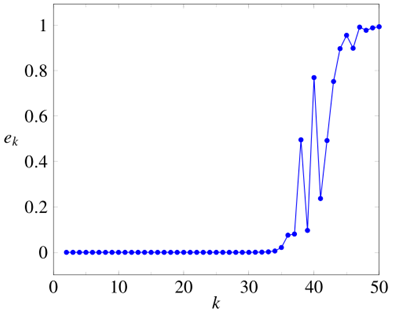
\includegraphics{qr-matlab-error.png}
        
    \end{figure}

    图中显示了 $ q_{k} $ 与前面列之间的正交性的偏差:

    $$
    e_{k}=\max _{1 \leq i<k}\left|q_{i}^{T} q_{k}\right|, \quad k=2, \ldots, n
    $$

    失去正交性是由于\textbf{浮点数存储的舍入误差}。
\end{example}

\section{Householder Algorithm}

Householder算法是QR分解常用的算法(MATLAB和Julia中的qr函数)。与Gram-Schmidt相比,对舍入误差更有鲁棒性。

Householder算法计算一个 “完整的” QR因数分解:
$$ A=\left[\begin{array}{ll}Q & \tilde{Q}\end{array}\right]\left[\begin{array}{l}R \\ 0\end{array}\right], \quad\left[\begin{array}{ll}Q & \tilde{Q}\end{array}\right]  是正交的矩阵$$

\begin{proof}
    $$
    \begin{aligned}
        A&=\left[\begin{array}{ll}Q & \tilde{Q}\end{array}\right]\left[\begin{array}{l}R \\ 0\end{array}\right]\\
        &=QR + \tilde{Q} 0 \\ 
        & = QR
    \end{aligned}
    $$
\end{proof}

完整的Q因子被构造成正交矩阵的乘积:
$$
\left[\begin{array}{ll}
Q & \tilde{Q}
\end{array}\right]=H_{1} H_{2} \cdots H_{n}
$$
每个 $ H_{i} \in \mathbb{R}^{m \times m} $ 是对称的正交的 “反射算子” (reflector)。


\subsection{反射算子}

\begin{theorem}
    $ H=I-2 v v^{T} $, 其中 $ \|v\|_{2}=1 $, $ H x $ 是 $ x $ 关于超平面 $ \left\{u \mid v^{T} u=0\right\} $ 反对称.

    $ H $ 是对称的 
    $$ H^{T}=H $$

$ H $ 是正交的 
$$ H^{T} H=I $$
\end{theorem}
    

\tikzset{every picture/.style={line width=0.75pt}} %set default line width to 0.75pt        



\tikzset{every picture/.style={line width=0.75pt}} %set default line width to 0.75pt        

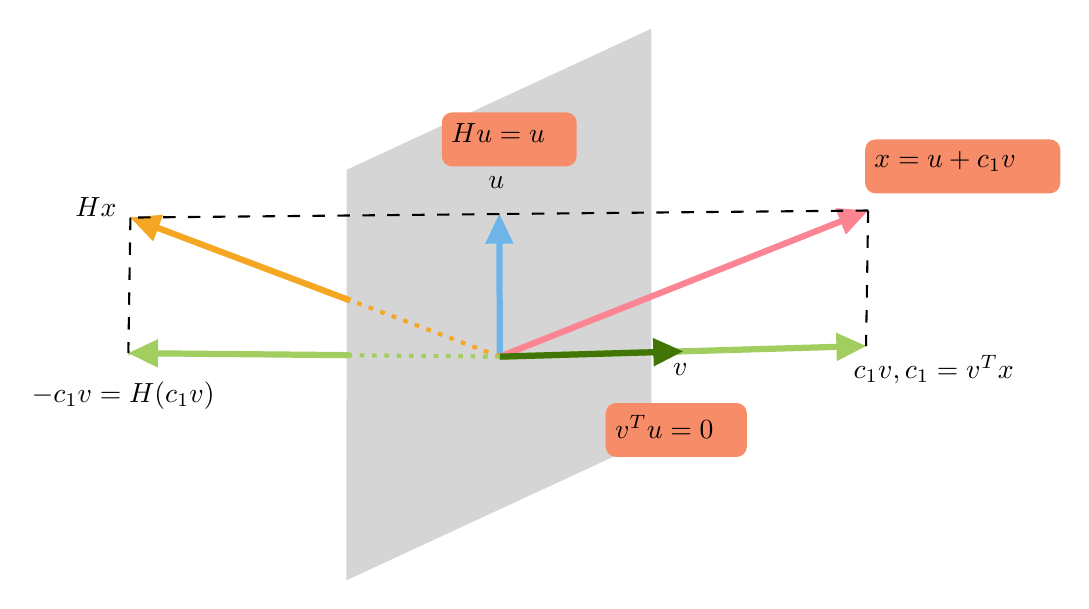
\begin{tikzpicture}[x=0.75pt,y=0.75pt,yscale=-1,xscale=1]
%uncomment if require: \path (0,300); %set diagram left start at 0, and has height of 300

%Shape: Parallelogram [id:dp7838939596356449] 
\draw  [color={rgb, 255:red, 0; green, 0; blue, 0 }  ,draw opacity=0 ][fill={rgb, 255:red, 213; green, 213; blue, 213 }  ,fill opacity=1 ] (386.97,225.43) -- (240.09,293.42) -- (240.13,95.65) -- (387,27.67) -- cycle ;
%Straight Lines [id:da6147749821862796] 
\draw [color={rgb, 255:red, 109; green, 180; blue, 232 }  ,draw opacity=1 ][line width=2.25]    (314,185.67) -- (313.74,121.96) ;
\draw [shift={(313.72,116.96)}, rotate = 449.76] [fill={rgb, 255:red, 109; green, 180; blue, 232 }  ,fill opacity=1 ][line width=0.08]  [draw opacity=0] (14.29,-6.86) -- (0,0) -- (14.29,6.86) -- cycle    ;
%Straight Lines [id:da41583656892756826] 
\draw [color={rgb, 255:red, 245; green, 166; blue, 35 }  ,draw opacity=1 ][line width=1.5]  [dash pattern={on 1.69pt off 2.76pt}]  (314,185.67) -- (136,118.67) ;
%Straight Lines [id:da16926502578383218] 
\draw [color={rgb, 255:red, 245; green, 166; blue, 35 }  ,draw opacity=1 ][line width=2.25]    (242,158.67) -- (140.68,120.43) ;
\draw [shift={(136,118.67)}, rotate = 380.66999999999996] [fill={rgb, 255:red, 245; green, 166; blue, 35 }  ,fill opacity=1 ][line width=0.08]  [draw opacity=0] (14.29,-6.86) -- (0,0) -- (14.29,6.86) -- cycle    ;
%Straight Lines [id:da9973542879627482] 
\draw [color={rgb, 255:red, 252; green, 132; blue, 147 }  ,draw opacity=1 ][line width=2.25]    (314,185.67) -- (486.78,117.1) ;
\draw [shift={(491.43,115.25)}, rotate = 518.35] [fill={rgb, 255:red, 252; green, 132; blue, 147 }  ,fill opacity=1 ][line width=0.08]  [draw opacity=0] (14.29,-6.86) -- (0,0) -- (14.29,6.86) -- cycle    ;
%Straight Lines [id:da33840798922577653] 
\draw [color={rgb, 255:red, 161; green, 206; blue, 94 }  ,draw opacity=1 ][line width=1.5]  [dash pattern={on 1.69pt off 2.76pt}]  (314,185.67) -- (135,183.96) ;
%Straight Lines [id:da7106398441661397] 
\draw [color={rgb, 255:red, 161; green, 206; blue, 94 }  ,draw opacity=1 ][line width=2.25]    (242,184.96) -- (140,184.01) ;
\draw [shift={(135,183.96)}, rotate = 360.53999999999996] [fill={rgb, 255:red, 161; green, 206; blue, 94 }  ,fill opacity=1 ][line width=0.08]  [draw opacity=0] (14.29,-6.86) -- (0,0) -- (14.29,6.86) -- cycle    ;
%Straight Lines [id:da3197102975021888] 
\draw [color={rgb, 255:red, 161; green, 206; blue, 94 }  ,draw opacity=1 ][line width=2.25]    (314,185.67) -- (485.43,180.69) ;
\draw [shift={(490.43,180.55)}, rotate = 538.3399999999999] [fill={rgb, 255:red, 161; green, 206; blue, 94 }  ,fill opacity=1 ][line width=0.08]  [draw opacity=0] (14.29,-6.86) -- (0,0) -- (14.29,6.86) -- cycle    ;
%Straight Lines [id:da07789590448724115] 
\draw  [dash pattern={on 4.5pt off 4.5pt}]  (136,118.67) -- (135,183.96) ;
%Straight Lines [id:da5486690595919534] 
\draw  [dash pattern={on 4.5pt off 4.5pt}]  (313.72,116.96) -- (136,118.67) ;
%Straight Lines [id:da1919773551202424] 
\draw  [dash pattern={on 4.5pt off 4.5pt}]  (491.43,115.25) -- (313.72,116.96) ;
%Straight Lines [id:da06488229558680647] 
\draw  [dash pattern={on 4.5pt off 4.5pt}]  (491.43,115.25) -- (490.43,180.55) ;
%Straight Lines [id:da5187220488118582] 
\draw [color={rgb, 255:red, 65; green, 117; blue, 5 }  ,draw opacity=1 ][line width=2.25]    (314,185.67) -- (397.22,183.25) ;
\draw [shift={(402.22,183.11)}, rotate = 538.3399999999999] [fill={rgb, 255:red, 65; green, 117; blue, 5 }  ,fill opacity=1 ][line width=0.08]  [draw opacity=0] (14.29,-6.86) -- (0,0) -- (14.29,6.86) -- cycle    ;

% Text Node
\draw (108,107.4) node [anchor=north west][inner sep=0.75pt]    {$\boldsymbol{Hx}$};
% Text Node
\draw (307,97.4) node [anchor=north west][inner sep=0.75pt]    {$u$};
% Text Node
\draw  [color={rgb, 255:red, 12; green, 12; blue, 12 }  ,draw opacity=0 ][fill={rgb, 255:red, 247; green, 140; blue, 105 }  ,fill opacity=1 ]  (286,73) .. controls (286,70.24) and (288.24,68) .. (291,68) -- (346,68) .. controls (348.76,68) and (351,70.24) .. (351,73) -- (351,89) .. controls (351,91.76) and (348.76,94) .. (346,94) -- (291,94) .. controls (288.24,94) and (286,91.76) .. (286,89) -- cycle  ;
\draw (289,72) node [anchor=north west][inner sep=0.75pt]   [align=left] {$\displaystyle \boldsymbol{Hu=u}$};
% Text Node
\draw (87,196.4) node [anchor=north west][inner sep=0.75pt]    {$\boldsymbol{-c_{1} v=H( c_{1} v)}$};
% Text Node
\draw  [color={rgb, 255:red, 0; green, 0; blue, 0 }  ,draw opacity=0 ][fill={rgb, 255:red, 247; green, 140; blue, 105 }  ,fill opacity=1 ]  (490,86) .. controls (490,83.24) and (492.24,81) .. (495,81) -- (579,81) .. controls (581.76,81) and (584,83.24) .. (584,86) -- (584,102) .. controls (584,104.76) and (581.76,107) .. (579,107) -- (495,107) .. controls (492.24,107) and (490,104.76) .. (490,102) -- cycle  ;
\draw (493,85.4) node [anchor=north west][inner sep=0.75pt]    {$\boldsymbol{x=u+c_{1} v}$};
% Text Node
\draw  [color={rgb, 255:red, 0; green, 0; blue, 0 }  ,draw opacity=0 ][fill={rgb, 255:red, 247; green, 140; blue, 105 }  ,fill opacity=1 ]  (365,213) .. controls (365,210.24) and (367.24,208) .. (370,208) -- (428,208) .. controls (430.76,208) and (433,210.24) .. (433,213) -- (433,229) .. controls (433,231.76) and (430.76,234) .. (428,234) -- (370,234) .. controls (367.24,234) and (365,231.76) .. (365,229) -- cycle  ;
\draw (368,212.4) node [anchor=north west][inner sep=0.75pt]    {$\boldsymbol{v}^{T}\boldsymbol{u} =0$};
% Text Node
\draw (483,183.4) node [anchor=north west][inner sep=0.75pt]    {$\boldsymbol{c_{1} v} ,\boldsymbol{c_{1} =v}^{T}\boldsymbol{x}$};
% Text Node
\draw (396,187.4) node [anchor=north west][inner sep=0.75pt]    {$\boldsymbol{v}$};


\end{tikzpicture}

\begin{proof}
    $$\begin{aligned}
        Hv &= (I-2 v v^{T}) (c_1 v) \\
        &= c_1 v - 2 v v^T c_1 v \\
        & = c_1 v - 2 c_1 v v^T v \\
        & = -c_1 v
    \end{aligned}$$

    $$\begin{aligned}
        Hu &= (I - 2 v v^T) u \\
        &= u - 2 v v^T u \\
        & = u \quad (v^T u = 0) 
    \end{aligned}$$

    $$\begin{aligned}
        Hx &= H(u + c_1v) \\
        &= u - c_1 v \\
        &= x - 2(v^Tx)v
    \end{aligned}$$
\end{proof}

矩阵向量积 $ H x $ 能化简为:
$$
H x=x-2\left(v^{T} x\right) v
$$

\subsubsection{$Hx$的算法复杂度}

\begin{theorem}
    如果 $ v $ 和 $ x $ 的长度是 $ p $, 复杂度是 $ 4 p $ flops 。
\end{theorem}


\subsection{构造反射算子}

给定非零p维向量 $ y=\left(y_{1}, y_{2}, \ldots, y_{p}\right) $, 定义

\begin{definition}
    $$w=\left[\begin{array}{c}
        y_{1}+\operatorname{sign}\left(y_{1}\right)\|y\|_{2} \\
        y_{2} \\
        \vdots \\
        y_{p}
        \end{array}\right]$$

    $$v=\frac{1}{\|w\|_{2}} w$$

    $\operatorname{sign}(x)$ 是符号函数, $\operatorname{sign}(0)=0$。
\end{definition}

\begin{theorem}
    向量 $ W $ 满足 $$ \|w\|_{2}^{2}=2 y^{T} w $$
\end{theorem}

$$
\begin{aligned}
    \|w\|_{2}^{2}&=w^{T} w\\
    &=2\left(\|y\|_{2}^{2}+\left|y_{1}\right|\|y\|_{2}\right)\\
    &=2 y^{T}\left(y+\operatorname{sign}\left(y_{1}\right)\|y\|_{2} e_{1}\right)\\
    &=2 y^{T} w 
\end{aligned}
$$

\begin{theorem}
    $$ H=I-2 \frac{w w^{T}}{\|w\|_{2}^{2}} $$
\end{theorem}

\begin{proof}
    $$ H=I-2 v v^{T}=I-2 \frac{w w^{T}}{\|w\|_{2}^{2}} \quad(v=\frac{1}{\|w\|_{2}} w) $$
\end{proof}

\begin{theorem}
    反射算子 $ H=I-2 v v^{T}=I-2 \frac{w w^{T}}{\|w\|_{2}^{2}} $ 将 $ y $ 映射为

   $$ H y = \left[\begin{array}{c}-\operatorname{sign}\left(y_{1}\right)\|y\|_{2} \\ 0 \\ \vdots \\ 0\end{array}\right] $$
\end{theorem}


\begin{proof}
    $$ 
\begin{aligned}
    H y&=y-\frac{2\left(w^{T} y\right)}{\|w\|_{2}^{2}} w\\
    &=y-w\\
    &=-\operatorname{sign}\left(y_{1}\right)\|y\|_{2} e_{1}\\
    &=\left[\begin{array}{c}-\operatorname{sign}\left(y_{1}\right)\|y\|_{2} \\ 0 \\ \vdots \\ 0\end{array}\right]
\end{aligned}
 $$
\end{proof}

即只保留一个元素的值,其余元素的值变为0. 又因为$H$是正交、对称的,它与向量正交化有一定联系。

\subsubsection{构造的反射算子几何意义}



\tikzset{every picture/.style={line width=0.75pt}} %set default line width to 0.75pt        



\tikzset{every picture/.style={line width=0.75pt}} %set default line width to 0.75pt        

\begin{tikzpicture}[x=0.75pt,y=0.75pt,yscale=-1,xscale=1]
%uncomment if require: \path (0,300); %set diagram left start at 0, and has height of 300

%Straight Lines [id:da029865045800250956] 
\draw    (118.48,198.47) -- (513.53,197.71) ;
%Straight Lines [id:da7648219943630132] 
\draw    (249.95,81.42) -- (422.95,297.42) ;
%Straight Lines [id:da0029727641306782626] 
\draw [color={rgb, 255:red, 252; green, 132; blue, 147 }  ,draw opacity=1 ][line width=2.25]    (344.25,197.82) -- (370.82,84.25) ;
\draw [shift={(371.96,79.38)}, rotate = 463.17] [fill={rgb, 255:red, 252; green, 132; blue, 147 }  ,fill opacity=1 ][line width=0.08]  [draw opacity=0] (14.29,-6.86) -- (0,0) -- (14.29,6.86) -- cycle    ;
%Straight Lines [id:da8143455838821552] 
\draw [color={rgb, 255:red, 245; green, 166; blue, 35 }  ,draw opacity=1 ][line width=2.25]    (344.25,197.82) -- (228.57,198.09) ;
\draw [shift={(223.57,198.11)}, rotate = 359.87] [fill={rgb, 255:red, 245; green, 166; blue, 35 }  ,fill opacity=1 ][line width=0.08]  [draw opacity=0] (14.29,-6.86) -- (0,0) -- (14.29,6.86) -- cycle    ;
%Straight Lines [id:da703987286749107] 
\draw  [dash pattern={on 4.5pt off 4.5pt}]  (297.77,138.74) -- (223.57,198.11) ;
%Straight Lines [id:da00886805291354964] 
\draw  [dash pattern={on 4.5pt off 4.5pt}]  (371.96,79.38) -- (297.77,138.74) ;
%Straight Lines [id:da1380735800367292] 
\draw [color={rgb, 255:red, 152; green, 195; blue, 245 }  ,draw opacity=1 ][line width=2.25]    (223.57,198.11) -- (368.05,82.5) ;
\draw [shift={(371.96,79.38)}, rotate = 501.34] [fill={rgb, 255:red, 152; green, 195; blue, 245 }  ,fill opacity=1 ][line width=0.08]  [draw opacity=0] (14.29,-6.86) -- (0,0) -- (14.29,6.86) -- cycle    ;

% Text Node
\draw (302.81,99.57) node [anchor=north west][inner sep=0.75pt]    {$w$};
% Text Node
\draw (159,208.4) node [anchor=north west][inner sep=0.75pt]    {$-\operatorname{sign}( y_{1}) \| y\| e_{1}$};
% Text Node
\draw (360.24,141.91) node [anchor=north west][inner sep=0.75pt]  [rotate=-357.61]  {$y$};
% Text Node
\draw (455,175) node [anchor=north west][inner sep=0.75pt]   [align=left] {坐标轴};
% Text Node
\draw (394,237) node [anchor=north west][inner sep=0.75pt]   [align=left] {超平面$\displaystyle \left\{x|w^{T} x=0\right\}$};


\end{tikzpicture}

关于超平面 $ \left\{x \mid w^{T} x=0\right\} $, 其法向量:
$$
v=\frac{w}{\|w\|_{2}}, w=y+\operatorname{sign}\left(y_{1}\right)\|y\|_{2} e_{1}
$$
反射算子$H$将 $ y $ 映射到向量 $ -\operatorname{sign}\left(y_{1}\right)\|y\|_{2} e_{1} $ 。

\subsection{Householder三角化}

计算反射算子 $ H_{1}, \ldots, H_{n} $ 将A简化为上三角矩阵形式:
$$
H_{n} H_{n-1} \cdots H_{1} A=\left[\begin{array}{l}
R \\
0
\end{array}\right]
$$

第k个步骤之后,矩阵 $ H_{k} H_{k-1} \ldots H_{1} A $ 具有以下结构

\tikzset{every picture/.style={line width=0.75pt}} %set default line width to 0.75pt        
对于 $ i>j $ 和 $ j \leq k $, 第 $ \mathrm{i}, \mathrm{j} $ 个位置的元素为零。

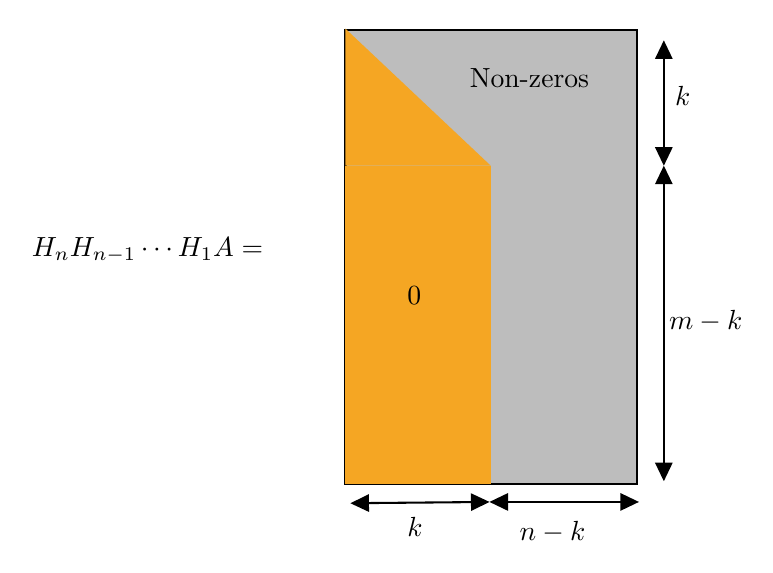
\begin{tikzpicture}[x=0.75pt,y=0.75pt,yscale=-1,xscale=1]
%uncomment if require: \path (0,300); %set diagram left start at 0, and has height of 300

%Shape: Rectangle [id:dp6272763265145869] 
\draw  [fill={rgb, 255:red, 189; green, 189; blue, 189 }  ,fill opacity=1 ] (313,30) -- (453.39,30) -- (453.39,248.71) -- (313,248.71) -- cycle ;
%Shape: Rectangle [id:dp1811444148627901] 
\draw  [color={rgb, 255:red, 0; green, 0; blue, 0 }  ,draw opacity=0 ][fill={rgb, 255:red, 245; green, 166; blue, 35 }  ,fill opacity=1 ] (313,95.38) -- (383,95.38) -- (383,248.71) -- (313,248.71) -- cycle ;
%Shape: Right Triangle [id:dp6024983200469929] 
\draw  [color={rgb, 255:red, 0; green, 0; blue, 0 }  ,draw opacity=0 ][fill={rgb, 255:red, 245; green, 166; blue, 35 }  ,fill opacity=1 ] (313,29.38) -- (383,95.38) -- (313,95.38) -- cycle ;

%Straight Lines [id:da17687674689557986] 
\draw    (466.39,38) -- (466.39,92.38) ;
\draw [shift={(466.39,95.38)}, rotate = 270] [fill={rgb, 255:red, 0; green, 0; blue, 0 }  ][line width=0.08]  [draw opacity=0] (8.93,-4.29) -- (0,0) -- (8.93,4.29) -- cycle    ;
\draw [shift={(466.39,35)}, rotate = 90] [fill={rgb, 255:red, 0; green, 0; blue, 0 }  ][line width=0.08]  [draw opacity=0] (8.93,-4.29) -- (0,0) -- (8.93,4.29) -- cycle    ;
%Straight Lines [id:da19218796013321793] 
\draw    (466.39,98.38) -- (466.39,244.38) ;
\draw [shift={(466.39,247.38)}, rotate = 270] [fill={rgb, 255:red, 0; green, 0; blue, 0 }  ][line width=0.08]  [draw opacity=0] (8.93,-4.29) -- (0,0) -- (8.93,4.29) -- cycle    ;
\draw [shift={(466.39,95.38)}, rotate = 90] [fill={rgb, 255:red, 0; green, 0; blue, 0 }  ][line width=0.08]  [draw opacity=0] (8.93,-4.29) -- (0,0) -- (8.93,4.29) -- cycle    ;
%Straight Lines [id:da4247865332087235] 
\draw    (318.39,257.97) -- (379.39,257.41) ;
\draw [shift={(382.39,257.38)}, rotate = 539.47] [fill={rgb, 255:red, 0; green, 0; blue, 0 }  ][line width=0.08]  [draw opacity=0] (8.93,-4.29) -- (0,0) -- (8.93,4.29) -- cycle    ;
\draw [shift={(315.39,258)}, rotate = 359.47] [fill={rgb, 255:red, 0; green, 0; blue, 0 }  ][line width=0.08]  [draw opacity=0] (8.93,-4.29) -- (0,0) -- (8.93,4.29) -- cycle    ;
%Straight Lines [id:da09293842736310576] 
\draw    (385.39,257.38) -- (451.39,257.38) ;
\draw [shift={(454.39,257.38)}, rotate = 180] [fill={rgb, 255:red, 0; green, 0; blue, 0 }  ][line width=0.08]  [draw opacity=0] (8.93,-4.29) -- (0,0) -- (8.93,4.29) -- cycle    ;
\draw [shift={(382.39,257.38)}, rotate = 0] [fill={rgb, 255:red, 0; green, 0; blue, 0 }  ][line width=0.08]  [draw opacity=0] (8.93,-4.29) -- (0,0) -- (8.93,4.29) -- cycle    ;

% Text Node
\draw (470.39,55.4) node [anchor=north west][inner sep=0.75pt]    {$k$};
% Text Node
\draw (467.39,163.78) node [anchor=north west][inner sep=0.75pt]    {$m-k$};
% Text Node
\draw (341.39,263.4) node [anchor=north west][inner sep=0.75pt]    {$k$};
% Text Node
\draw (395.39,265.4) node [anchor=north west][inner sep=0.75pt]    {$n-k$};
% Text Node
\draw (160.39,128.4) node [anchor=north west][inner sep=0.75pt]    {$H_{n} H_{n-1} \cdots H_{1} A=$};
% Text Node
\draw (341.39,152.4) node [anchor=north west][inner sep=0.75pt]    {$\boldsymbol{0}$};
% Text Node
\draw (371.39,47) node [anchor=north west][inner sep=0.75pt]   [align=left] {Non-zeros};


\end{tikzpicture}



$$ A=\left[\begin{array}{llllllll}X & X & X & X & X & X & X & X \\ X & X & X & X & X & X & X & X \\ X & X & X & X & X & X & X & X \\ X & X & X & X & X & X & X & X \\ X & X & X & X & X & X & X & X \\ X & X & X & X & X & X & X & X \\ X & X & X & X & X & X & X & X \\ X & X & X & X & X & X & X & X\end{array}\right] $$

在第一次处理之后,第一列只剩下第一个元素不为0.

$$H_1A = A_{1}=\left[\begin{array}{llllllll}X & X & X & X & X & X & X & X \\ 0 & X & X & X & X & X & X & X \\ 0 & X & X & X & X & X & X & X \\ 0 & X & X & X & X & X & X & X \\ 0 & X & X & X & X & X & X & X \\ 0 & X & X & X & X & X & X & X \\ 0 & X & X & X & X & X & X & X \\ 0 & X & X & X & X & X & X & X\end{array}\right] $$

第二次处理对于$H_1A_{2:m, 1:n}$($A_{1_{2:m, 1:n} }  $)进行处理。

$$H_2A_1= A_{2}=\left[\begin{array}{cccccccc}X & X & X & X & X & X & X & X \\ 0 & X & X & X & X & X & X & X \\ 0 & 0 & X & X & X & X & X & X \\ 0 & 0 & X & X & X & X & X & X \\ 0 & 0 & X & X & X & X & X & X \\ 0 & 0 & X & X & X & X & X & X \\ 0 & 0 & X & X & X & X & X & X \\ 0 & 0 & X & X & X & X & X & X\end{array}\right] $$

\begin{theorem}
    第$k$个步骤之后,矩阵 $ H_{k} H_{k-1} \ldots H_{1} A $ 具有以下结构:

对于 $ i>j $ 和 $ j \leq k $, 第 $ \mathrm{i}, \mathrm{j} $ 个位置的元素为零.
\end{theorem}


下面的算法用 $ \left[\begin{array}{l}R \\ 0\end{array}\right] $ 来代替 $ A \in \mathbb{R}^{m \times n} $.



\begin{center}
    \tikzset{every picture/.style={line width=0.75pt}} %set default line width to 0.75pt        

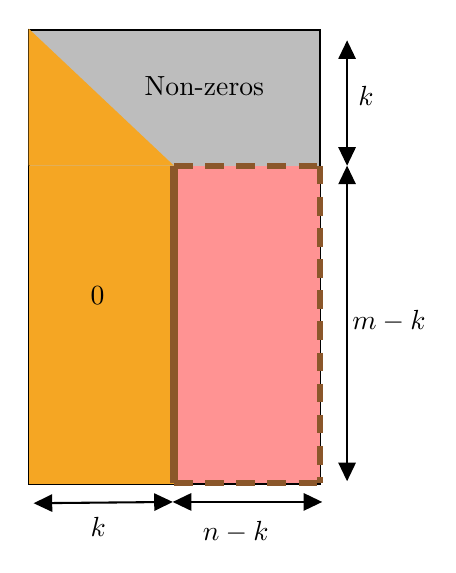
\begin{tikzpicture}[x=0.75pt,y=0.75pt,yscale=-1,xscale=1]
%uncomment if require: \path (0,300); %set diagram left start at 0, and has height of 300

%Shape: Rectangle [id:dp6871792923402225] 
\draw  [fill={rgb, 255:red, 189; green, 189; blue, 189 }  ,fill opacity=1 ] (333,28) -- (473.39,28) -- (473.39,246.71) -- (333,246.71) -- cycle ;
%Shape: Rectangle [id:dp8707939685410495] 
\draw  [color={rgb, 255:red, 0; green, 0; blue, 0 }  ,draw opacity=0 ][fill={rgb, 255:red, 245; green, 166; blue, 35 }  ,fill opacity=1 ] (333,93.38) -- (403,93.38) -- (403,246.71) -- (333,246.71) -- cycle ;
%Shape: Right Triangle [id:dp15297612966191965] 
\draw  [color={rgb, 255:red, 0; green, 0; blue, 0 }  ,draw opacity=0 ][fill={rgb, 255:red, 245; green, 166; blue, 35 }  ,fill opacity=1 ] (333,27.38) -- (403,93.38) -- (333,93.38) -- cycle ;

%Straight Lines [id:da37642223834770605] 
\draw    (486.39,36) -- (486.39,90.38) ;
\draw [shift={(486.39,93.38)}, rotate = 270] [fill={rgb, 255:red, 0; green, 0; blue, 0 }  ][line width=0.08]  [draw opacity=0] (8.93,-4.29) -- (0,0) -- (8.93,4.29) -- cycle    ;
\draw [shift={(486.39,33)}, rotate = 90] [fill={rgb, 255:red, 0; green, 0; blue, 0 }  ][line width=0.08]  [draw opacity=0] (8.93,-4.29) -- (0,0) -- (8.93,4.29) -- cycle    ;
%Straight Lines [id:da1511742331917798] 
\draw    (486.39,96.38) -- (486.39,242.38) ;
\draw [shift={(486.39,245.38)}, rotate = 270] [fill={rgb, 255:red, 0; green, 0; blue, 0 }  ][line width=0.08]  [draw opacity=0] (8.93,-4.29) -- (0,0) -- (8.93,4.29) -- cycle    ;
\draw [shift={(486.39,93.38)}, rotate = 90] [fill={rgb, 255:red, 0; green, 0; blue, 0 }  ][line width=0.08]  [draw opacity=0] (8.93,-4.29) -- (0,0) -- (8.93,4.29) -- cycle    ;
%Straight Lines [id:da9300057482807336] 
\draw    (338.39,255.97) -- (399.39,255.41) ;
\draw [shift={(402.39,255.38)}, rotate = 539.47] [fill={rgb, 255:red, 0; green, 0; blue, 0 }  ][line width=0.08]  [draw opacity=0] (8.93,-4.29) -- (0,0) -- (8.93,4.29) -- cycle    ;
\draw [shift={(335.39,256)}, rotate = 359.47] [fill={rgb, 255:red, 0; green, 0; blue, 0 }  ][line width=0.08]  [draw opacity=0] (8.93,-4.29) -- (0,0) -- (8.93,4.29) -- cycle    ;
%Straight Lines [id:da8104730881110522] 
\draw    (405.39,255.38) -- (471.39,255.38) ;
\draw [shift={(474.39,255.38)}, rotate = 180] [fill={rgb, 255:red, 0; green, 0; blue, 0 }  ][line width=0.08]  [draw opacity=0] (8.93,-4.29) -- (0,0) -- (8.93,4.29) -- cycle    ;
\draw [shift={(402.39,255.38)}, rotate = 0] [fill={rgb, 255:red, 0; green, 0; blue, 0 }  ][line width=0.08]  [draw opacity=0] (8.93,-4.29) -- (0,0) -- (8.93,4.29) -- cycle    ;
%Shape: Rectangle [id:dp3957948372583875] 
\draw  [color={rgb, 255:red, 0; green, 0; blue, 0 }  ,draw opacity=0 ][fill={rgb, 255:red, 255; green, 147; blue, 147 }  ,fill opacity=1 ] (403,93.38) -- (473.39,93.38) -- (473.39,246.42) -- (403,246.42) -- cycle ;
%Straight Lines [id:da6423678439002216] 
\draw [color={rgb, 255:red, 139; green, 87; blue, 42 }  ,draw opacity=1 ][line width=3]    (403,93.38) -- (403,246.42) ;
%Straight Lines [id:da15094884239960105] 
\draw [color={rgb, 255:red, 139; green, 87; blue, 42 }  ,draw opacity=1 ][line width=2.25]  [dash pattern={on 6.75pt off 4.5pt}]  (403,93.38) -- (473.39,93.38) ;
%Straight Lines [id:da6820341280353248] 
\draw [color={rgb, 255:red, 139; green, 87; blue, 42 }  ,draw opacity=1 ][line width=2.25]  [dash pattern={on 6.75pt off 4.5pt}]  (473.39,93.38) -- (473.39,246.42) ;
%Straight Lines [id:da3968465055227026] 
\draw [color={rgb, 255:red, 139; green, 87; blue, 42 }  ,draw opacity=1 ][line width=2.25]  [dash pattern={on 6.75pt off 4.5pt}]  (403,246.42) -- (473.39,246.42) ;

% Text Node
\draw (490.39,53.4) node [anchor=north west][inner sep=0.75pt]    {$k$};
% Text Node
\draw (487.39,161.78) node [anchor=north west][inner sep=0.75pt]    {$m-k$};
% Text Node
\draw (361.39,261.4) node [anchor=north west][inner sep=0.75pt]    {$k$};
% Text Node
\draw (415.39,263.4) node [anchor=north west][inner sep=0.75pt]    {$n-k$};
% Text Node
\draw (361.39,150.4) node [anchor=north west][inner sep=0.75pt]    {$\boldsymbol{0}$};
% Text Node
\draw (387.39,49) node [anchor=north west][inner sep=0.75pt]   [align=left] {Non-zeros};


\end{tikzpicture}
\end{center}


\begin{algorithm}[htbp]
    \caption{Householder算法}

    \For(){$k$ in $1:n$}{
        令 $ y=A_{k: m, k} \in \mathbb{R}^{m-k+1} $, 计算向量 $ v_{k} $
    $$ w=y+\operatorname{sign}\left(y_{1}\right)\|y\| e_{1}, \quad v_{k}=\frac{1}{\|w\|} w $$\;
    将 $ A_{k: m, k: n} \in \mathbb{R}^{(m-k+1) \times(n-k+1)} $ 与反射矩阵 $ I-2 v_{k} v_{k}^{T} $ 相乘
    $$ A_{k: m, k: n}:=A_{k: m, k: n}-2 v_{k}\left(v_{k}^{T} A_{k: m, k: n}\right) $$\;

    }
    
\end{algorithm}

\begin{proof}
    在步骤2中,将 $ A_{k: m, k: n} $ 与反射算子 $ I-2 v_{k} v_{k}^{T} $ 相乘

$$ \left(I-2 v_{k} v_{k}^{T}\right) A_{k: m, k: n}=A_{k: m, k: n}-2 v_{k}\left(v_{k}^{T} A_{k: m, k: n}\right) $$

等价于用 $ H_{k} \in \mathbb{R}^{m \times m} $ 乘以 $ A $

$$ H_{k}=\left[\begin{array}{cc}I & 0 \\ 0 & I-2 v_{k} v_{k}^{T}\end{array}\right]=I-2\left[\begin{array}{c}0 \\ v_{k}\end{array}\right]\left[\begin{array}{l}0 \\ v_{k}\end{array}\right]^{T} $$

算法将下列矩阵来代替 $ A $
$$
\left[\begin{array}{c}
R \\
0
\end{array}\right]
$$

返回向量 $ v_{1}, \ldots, v_{n} $, 其中 $ v_{k} $ 的长度为 $ m-k+1 $ 。
\end{proof}


\subsection{An Example for Householder Algorithm}

\begin{problem}
    $$ A=\left[\begin{array}{rrr}-1 & -1 & 1 \\ 1 & 3 & 3 \\ -1 & -1 & 5 \\ 1 & 3 & 7\end{array}\right]=H_{1} H_{2} H_{3}\left[\begin{array}{l}R \\ 0\end{array}\right] $$

    计算反射算子 $ H_{1}, H_{2}, H_{3} $ 来将矩阵$A$三角化

    $$ H_{3} H_{2} H_{1} A=\left[\begin{array}{ccc}R_{11} & R_{12} & R_{13} \\ 0 & R_{22} & R_{23} \\ 0 & 0 & R_{33} \\ 0 & 0 & 0\end{array}\right] $$

    $R$的第一列:计算将$A$的第一列映射到$e_1$乘积的反射算子

    $$
y=\left[\begin{array}{r}
-1 \\
1 \\
-1 \\
1
\end{array}\right], \quad w=y-\|y\|_{2} e_{1}=\left[\begin{array}{r}
-3 \\
1 \\
-1 \\
1
\end{array}\right], \quad v_{1}=\frac{1}{\|w\|_{2}} w=\frac{1}{2 \sqrt{3}}\left[\begin{array}{r}
-3 \\
1 \\
-1 \\
1
\end{array}\right]
$$

用 $I-2 v_{1} v_{1}^{T}$ 和$A$的乘积代替$A$:
$$
A:=\left(I-2 v_{1} v_{1}^{T}\right) A=\left[\begin{array}{ccc}
2 & 4 & 2 \\
0 & 4 / 3 & 8 / 3 \\
0 & 2 / 3 & 16 / 3 \\
0 & 4 / 3 & 20 / 3
\end{array}\right]
$$

$R$的第二列:计算将 $ A_{2: 4,2} $ 映射到 $ e_{1} $ 乘积的反射算子

$$y=\left[\begin{array}{l}
    4 / 3 \\
    2 / 3 \\
    4 / 3
    \end{array}\right], \quad w=y+\|y\|_{2} e_{1}=\left[\begin{array}{r}
    10 / 3 \\
    2 / 3 \\
    4 / 3
    \end{array}\right], \quad v_{2}=\frac{1}{\|w\|_{2}} w=\frac{1}{\sqrt{30}}\left[\begin{array}{l}
    5 \\
    1 \\
    2
    \end{array}\right]
$$

用 $I-2 v_{2} v_{2}^{T}$ 和 $A_{2: 4,2: 3}$ 的乘积代替 $A_{2: 4,2: 3}$ :
$$
A:=\left[\begin{array}{cc}
1 & 0 \\
0 & I-2 v_{2} v_{2}^{T}
\end{array}\right] A=\left[\begin{array}{rrr}
2 & 4 & 2 \\
0 & -2 & -8 \\
0 & 0 & 16 / 5 \\
0 & 0 & 12 / 5
\end{array}\right]
$$

$R$的第三列:计算将$ A_{3: 4,3} $映射到$e_1$乘积的反射算子

$$y=\left[\begin{array}{l}
    16 / 5 \\
    12 / 5
    \end{array}\right], \quad w=y+\|y\|_{2} e_{1}=\left[\begin{array}{c}
    36 / 5 \\
    12 / 5
    \end{array}\right], \quad v_{3}=\frac{1}{\|w\|_{2}} w=\frac{1}{\sqrt{10}}\left[\begin{array}{l}
    3 \\
    1
    \end{array}\right]
$$

用 $I-2 v_{3} v_{3}^{T}$ 和 $A_{3: 4,3}$ 的乘积代替 $A_{3: 4,3}$ :
$$
A:=\left[\begin{array}{cc}
I & 0 \\
0 & I-2 v_{3} v_{3}^{T}
\end{array}\right] A=\left[\begin{array}{rrr}
2 & 4 & 2 \\
0 & -2 & -8 \\
0 & 0 & -4 \\
0 & 0 & 0
\end{array}\right]
$$


    $$ \begin{aligned} H_{3} H_{2} H_{1} A &=\left[\begin{array}{cc}I_{2} & 0 \\ 0 & I_{2}-2 v_{3} v_{3}^{T}\end{array}\right]\left[\begin{array}{cc}I_{1} & 0 \\ 0 & I_{3}-2 v_{2} v_{2}^{T}\end{array}\right]\left(I_{4}-2 v_{1} v_{1}^{T}\right) A \\ &=\left[\begin{array}{cc}I_{2} & 0 \\ 0 & I_{2}-2 v_{3} v_{3}^{T}\end{array}\right]\left[\begin{array}{cc}I_{1} & 0 \\ 0 & I_{3}-2 v_{2} v_{2}^{T}\end{array}\right]\left[\begin{array}{ccc}2 & 4 & 2 \\ 0 & 4 / 3 & 8 / 3 \\ 0 & 2 / 3 & 16 / 3 \\ 0 & 4 / 3 & 20 / 3\end{array}\right] \\ &=\left[\begin{array}{cc}I_{2} & 0 \\ 0 & I_{2}-2 v_{3} v_{3}^{T}\end{array}\right]\left[\begin{array}{rrr}2 & 4 & 2 \\ 0 & -2 & -8 \\ 0 & 0 & 16 / 5 \\ 0 & 0 & 12 / 5\end{array}\right] \\ &=\left[\begin{array}{rrr}2 & 4 & 2 \\ 0 & -2 & -8 \\ 0 & 0 & -4 \\ 0 & 0 & 0\end{array}\right] \end{aligned} $$
\end{problem}

\subsection{Complexity of Householder Algorithm}

Householder方法第$k$次循环的复杂度:

\begin{itemize}
    \item $ v_{k}^{T} A_{k: m, k: n} $ 的乘积: $ (2(\mathrm{~m}-\mathrm{k}+1)-1)(\mathrm{n}-\mathrm{k}+1) $ flops
    \item $ v_{k} $ 的外积: $ (m-k+1)(n-k+1) $ flops
    \item $ A_{k: m, k: n} $ 的减法: $ (\mathrm{m}-\mathrm{k}+1)(\mathrm{n}-\mathrm{k}+1) $ flops
\end{itemize}

第$k$次循环的总和: $ 4(\mathrm{~m}-\mathrm{k}+1)(\mathrm{n}-\mathrm{k}+1) $ flops

计算 $ R $ 和 $ v_{1}, \ldots, v_{n} $ 的总复杂度

$$ \begin{aligned} \sum_{k=1}^{n} 4(m-k+1)(n-k+2) & \approx \int_{0}^{n} 4(m-t)(n-t+1) d t \\ & \approx 2 m n^{2}-\frac{2}{3} n^{3} \text { flops } \end{aligned} $$

\section{$Q$因子}

Householder算法返回向量 $ v_{1}, \ldots, v_{n} $, 其定义为:

\begin{definition}[ $ v_{1}, \ldots, v_{n} $ 的完整表示]
   $$
\left[\begin{array}{ll}
Q & \tilde{Q}
\end{array}\right]=H_{1} H_{2} \cdots H_{n}
$$ 
\end{definition}

通常不需计算矩阵 $ \left[\begin{array}{ll}Q & \tilde{Q}\end{array}\right] $ 。向量 $ v_{1}, \ldots, v_{n} $ 是 $ \left[\begin{array}{ll}Q & \tilde{Q}\end{array}\right] $ 简单表示(economical representation)。

\begin{theorem}
    $ \left[\begin{array}{ll}Q & \tilde{Q}\end{array}\right] $ 或其转置的乘积可以计算为:
$$
\begin{array}{c}
{\left[\begin{array}{cc}
Q & \tilde{Q}
\end{array}\right] x=H_{1} H_{2} \cdots H_{n} x} \\
{\left[\begin{array}{ll}
Q & \tilde{Q}
\end{array}\right]^{T} y=H_{n} H_{n-1} \cdots H_{1} y}
\end{array}
$$
\end{theorem}

\begin{definition}
    矩阵-向量积 $ H_{k} x $ 定义为:
$$
H_{k} x=\left[\begin{array}{cc}
I_{k-1} & 0 \\
0 & I-2 v_{k} v_{k}^{T}
\end{array}\right]\left[\begin{array}{c}
x_{1: k-1} \\
x_{k: m}
\end{array}\right]=\left[\begin{array}{c}
x_{1: k-1} \\
x_{k: m}-2\left(v_{k}^{T} x_{k: m}\right) v_{k}
\end{array}\right]
$$
\end{definition}

\subsection{矩阵-向量积 $ H_{k} x $算法复杂度}

$ H_{k} x $ 乘积的复杂度为: $ 4(\mathrm{~m}-\mathrm{k}+1) $ flops。

$H_{1} H_{2}, \ldots H_{n} $或其转置的乘积的复杂度为: 

$$ \sum_{k=1}^{n} 4(m-k+1) \approx 4 m n-2 n^{2}  \text{ flops}$$

其复杂度约等于$m \times n$矩阵的矩阵-向量乘积($2mn$ flops)。 